%% ============================================================
%%  Chapter 2 - Artificial Intelligence and Machine Learning
%%  Simplified, no heavy formulas. All citations verified.
%% ============================================================

\chapter{Artificial Intelligence and Machine Learning}
\label{chap:ai}

\section{Introduction}

While "artificial intelligence" is quite broad, much of what people call AI in everyday language is a smaller subset: machine learning. Instead of someone sitting down and writing out a few if-then statements-"if this comes from this IP address and hits this port more than ten times a second, block it" we give a learning system a bunch of training examples and let it figure out the rule based on the data. This move from programmed logic to learning logic makes ML very powerful for tasks like intrusion detection. Attackers rarely declare their intentions upfront in a form that an rule-designer would recognize but they do create their traffic in a way that’s statistically regular, and the machine learning model picks up this pattern.
This section aims to remain mostly non-technical. I won't spend time on deriving the mathematics for each algorithm, but rather on providing enough background to fully understand Chapter~\ref{chap:ids}.
Section~\ref{sec:ml_types} discusses how the learning system is characterized by what it has learned from. 
Section~\ref{sec:ml_pipeline} explores the typical workflow. 
Section~\ref{sec:classical_ml} provides an overview of classical ML algos, those that predated and still inform deep learning, namely Random Forest (used here in baseline configurations). Section~\ref{sec:deep_learning} demystifies deep learning and why it became so dominant. We’ll end this section in Section~\ref{sec:xai} with an overview of explainability because making the model’s decision process clear to human eyes is another key goal of this project.

% ────────────────────────────────────────────────────────────
\section{How Machine Learning Systems Learn}
\label{sec:ml_types}

There is not simply “a way of doing“ machine learning. A variety of approaches can be taken, as we have seen, depending on your task and available data resources. A systematic review of the state-of-the-art by Alloghani et al. From 2020 analysed 84 research papers published between 2015 and 2018 and provided the key ML tasks categories: decision trees, support vector machines, and Naive Bayes was identified as the highest utilized supervised algorithms within these papers \cite{alloghani2020systematic}.

\subsection{Supervised learning}

With supervised learning, every data point in the training set also has an associated label a "ground truth" of the "right answer". If you are building a spam filter, each email in the training set is classified as either "spam" or "not spam." If you are building a brute-force attack detector, each flow in your training set will be labeled as "benign" or "brute-force." The training procedure for the model is to induce a pattern that connects the input (email or flow) to its correct classification, correcting it each time it fails to.

This methodology is pervasive in IDS research, primarily because datasets such as the CICIDS-2017 contain explicit labels, someone conducted attacks, generated traffic for each attack type, and then meticulously identified and logged which network flow was associated with which attack type \cite{sharafaldin2018cicids}. Without these annotations, the supervised learning approach simply has nothing to learn from.

\subsection{Unsupervised learning}
Unsupervised learning don't need labels. The model is simply provided with a set of data and asked to discover structures within this data, it should distinguish and cluster related data together, or detect data points that are significantly different from the main data pattern. In the context of network intrusion detection, this could mean the unsupervised model will learn how "normal" traffic appears to be and consequently identify any deviation from that pattern without receiving any beforehand information about the nature of an attack. 

While it is true that unsupervised learning can potentially discover novel attacks-which is indeed one of its undeniable merits, an idea further supported by Talaei Khoei and Kaabouch's comparison between unsupervised and supervised models with various intrusion detection data sets-the cost it has to pay in terms of performance is high \cite{khoei2023comparative}. 

Specifically, "different from normal" is not equivalent to "malicious". An unnormal but legitimate traffic spike might appear indistinguishable from a malicious attack from the model’s perspective, hence the relatively large rates of false alerts that are commonly associated with such models. This very reason why unsupervised learning is not the primary learning methodology of this project.

\subsection{A quick note on semi-supervised learning}

Of course there's a middle-ground: semi-supervised learning where a model is supplied with only a small pool of labelled data, but far larger amounts of unlabelled. The model uses the labelled examples to anchor and the unlabelled data to help flesh out its understanding. Mvula et al., in their 2024 survey of semi-supervised learning methods in cyber-security, explain semi-supervised learning as a direct response to what they see as a fundamental structural problem of our field: labelled traffic samples are difficult and costly to generate, while the volume of unlabelled traffic generated is enormous, and semi-supervised techniques make a reasonable attempt to exploit these resource disparities \cite{mvula2024semisupervised}. This is particularly pertinent in cyber-security where hand-labeling attack traffic relies on scarce, time-consuming expert human intervention.

% ────────────────────────────────────────────────────────────
\section{How a Model Actually Gets Built}
\label{sec:ml_pipeline}

We talk of training the model as if it were one step. The reality involves a sequence of rather tedious steps. Most of the actual work in an ML project involves activities which occur before the model ever gets to see any data at all.

\begin{enumerate}[label=\arabic*.]
  \item \textbf{Collect the data:} Which in our project, will include the CICIDS-2017 CSV files, along with some real traffic captured in lab.

  \item \textbf{Turn it into numbers:} No one can read a packet capture straight. The raw network traffic is first translated into a table of numerical features, such as the count of packets in the flow, duration of the flow, set flags, and many others. This process is named feature extraction and in this particular case, the feature extraction is done using CICFlowMeter, the tool which was used to generate the CICIDS-2017 features before.
  \item \textbf{Split the data:} Data splits into a train portion(this is what the model learns on) and a test set portion (a set kept back from the model, to test how it will generalize to data it hasn't seen). There are no hard rules here but usually, you will see a split of something like 70/30 or 80/20, depending on the volume of data you have to begin with.

  \item \textbf{Train:} The model goes through the training data multiple times, tuning itself each pass to minimize its errors. The specific details of "tuning itself" depend on the algorithm for Random Forests it means growing trees, for neural nets it means nudging around numerical weights.

  \item \textbf{Test:} After the training, the model is used on the test set that it didn't even touch during the learning process. This is the only just way to determine if the model truly understood, rather than just learning by memorising.

  \item \textbf{Deploy:} If the performance is adequate then the model goes in to real time deployment in this case classifying incoming live traffic streams as they are ingested.
\end{enumerate}

\subsection{How do you know if it's any good?}

After training a model, you're going to need some way to score it, and "accuracy" alone is a minefield. Umer et al, in a survey of ML-based intrusion detection for industrial control systems, note that IDS datasets are most always a skewed class problem: most of the time normal traffic forms over 90\% of the dataset, and so a classifier which labels every example as normal - without inspecting it - would get over 90\% just from accuracy \cite{umer2022ics}. CICIDS-2017 does indeed have this skew, so it becomes crucial to consider other measures.

These additional measures can be calculated from the four possible outcomes of a classification, illustrated in a confusion matrix in table \ref{tab:confusion_matrix}:

\begin{table}[H]
  \centering
  \caption{The four possible outcomes of a binary classification framed for IDS}
  \label{tab:confusion_matrix}
  \renewcommand{\arraystretch}{1.5}
  \begin{tabular}{ll cc}
    \toprule
    & & \multicolumn{2}{c}{\textbf{Actual traffic}} \\
    & & Attack & Benign \\
    \midrule
    \multirow{2}{*}{\textbf{Model says}}
      & Attack  & True Positive (TP) & False Positive (FP) \\
      & Benign  & False Negative (FN) & True Negative (TN) \\
    \bottomrule
  \end{tabular}
\end{table}

A false positive is an harmless flow that you have identified as a attack (in other words an alarm that should never have happened). A false negative is a real attack that you did not notice (a far more serious error from a security point of view).

\begin{itemize}
  \item \textbf{Precision : }  Of everything the model flagged as an attack, what was one? TP/(TP + FP). If precision is low there is a lot of false alarms
  
  \item \textbf{Recall : } (sometimes called detection rate) - how many of all the real
 attacks did the model detect? TP / (TP + FN). Low recall means attacks get through.
 
  \item \textbf{F1 score : } The single metric that finds the optimal sweet spot between precision and recall, a metric used for comparing models instead of trying to remember the 2 of them separately.
\end{itemize}

The measures of precision and recall typically come with an inverse relationship with each other: tune a model to catch more of the attacks (high recall) and it will be likely to classify many legitimate activities as attacks too (low precision). This tradeoff depends on the particular use-case rather than pure math; when using an intrusion detection system (IDS) missing real attacks are often deemed worse than a few false positives, but high false positives can make analysts tune out altogether \cite{umer2022ics}.

% ────────────────────────────────────────────────────────────
\section{Classical Algorithms: Trees and Forests}
\label{sec:classical_ml}

In days before deep learning took center stage, several very simple algorithms were responsible for most of the effort put forth in applied machine learning, and many still continue that task not because they have historical significance as predecessors, but because they work they are efficient, they’re understandable, and oftentimes just as accurate as models that are magnitudes more complex. This is not simply an argument based on practicalities: A comparative controlled test of DL and classical models, conducted in 2025, comparing model performance on network intrusion data shows CNN and LSTM models perform about 98\%, whereas a Random Forest performing the exact same task achieved a 99.9\% score; classical models perform better here \cite{ali2025dlvsml}. While the result of course depends on the specific problem and dataset, it’s a concrete outcome that’s very common in the literature, and one reason that we can see a Random Forest model as a first pass approach and not a “compromise”.
 
\subsection{Decision trees}
 
A decision tree acts as it sounds, you’re asking a series of questions of the input, and based on the answer you traverse one path in the tree to another question, until you eventually come to a conclusion: “Is the destination port 22? If yes, do I have more than one connection attempt per second from this source? If yes, flag brute force.” The decision tree idea itself originates from Quinlan’s ID3 algorithm, which in essence builds a tree, each step of the way, selecting the question that best separates the available examples into their respective categories \cite{quinlan1986id3}.
 
What a thing like this looks like is illustrated in a simplified manner in figure~\ref{fig:decision_tree} for a type of decision like those that our project’s IDS must make.
 
\begin{figure}[H]
  \centering
  \IfFileExists{figures/decision_tree_example.png}{%
    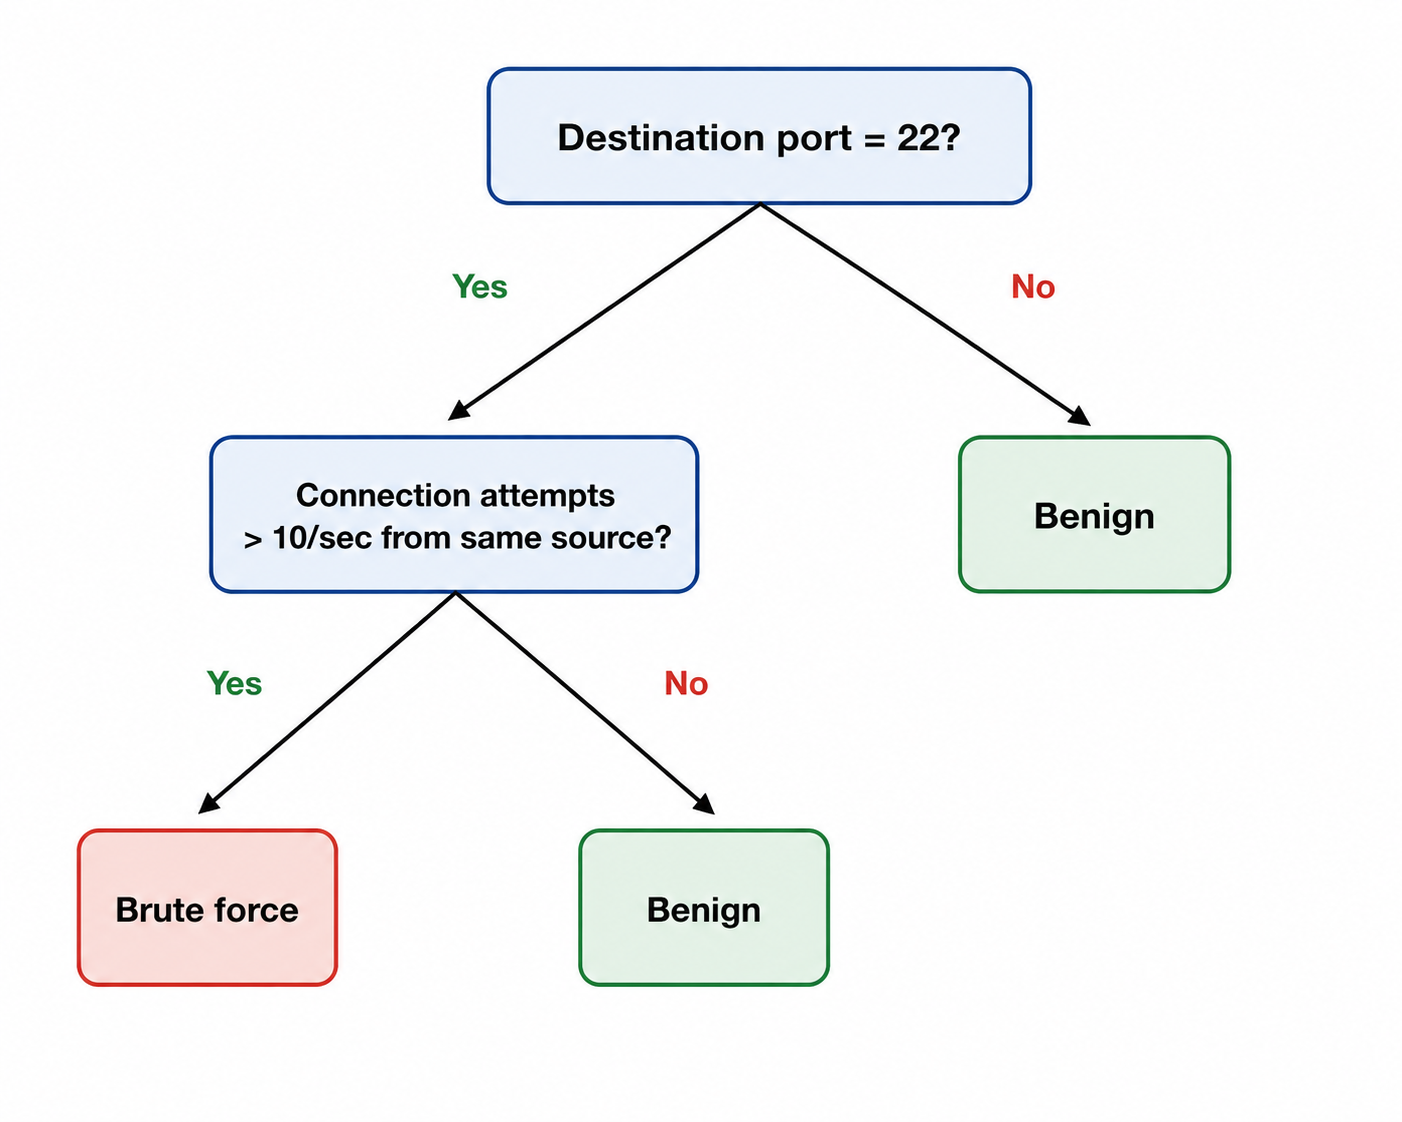
\includegraphics[width=0.75\textwidth]{figures/decision_tree_example.png}%
  }{%
    \fbox{\parbox{0.78\textwidth}{\centering\vspace{1.2cm}
    \texttt{[Figure: decision\_tree\_example.png, to be created]}\\[4pt]
    \small A simple original diagram: a root node asking "Destination port = 22?",
    branching to a node asking "Connection attempts $>$ 10/sec from same source?",
    branching down to two leaf nodes labelled "Brute force" and "Benign." Draw
    directly in draw.io, PowerPoint, or a tikzpicture, no external image needed.
    \vspace{1.2cm}}}%
  }
  \caption{Simplified decision tree for flagging SSH brute-force traffic}
  \label{fig:decision_tree}
\end{figure}
 
What is nice about a single tree is that you can literally just read it to see exactly why each decision was made. What is unfortunate, as identified by Quinlan himself in a discussion of the approach, is that because a tree built greedily one split at a time can never “undo” a mistake it made early on when it’s able to see more data \cite{quinlan1986id3}, it can sometimes be “overfitted” to peculiarities of its particular training set, so that tiny changes in training data result in a considerably different tree.
 
\subsection{Random Forest}
 
The Random Forest overcomes this instability by training multiple (often several hundred) trees instead of one and averaging over their predictions. To train each tree, we either use a slightly different random sample of the training data, or we randomly constrain the set of features to use at each split. In the paper that introduced the algorithm, Leo Breiman described the forest as a collection of tree predictors where each tree is grown from its own independently sampled random vector, and he proved that the generalization error of the ensemble settles towards a limit as more trees are added rather than growing worse -- adding trees cannot overfit the forest \cite{breiman2001random}.

We represent this concept schematically in Figure~\ref{fig:random_forest}: the flow through a number of similar-looking trees is run, and the result is the one which receives a majority vote among all the trees.
 
\begin{figure}[H]
  \centering
  \IfFileExists{figures/random_forest_voting.png}{%
    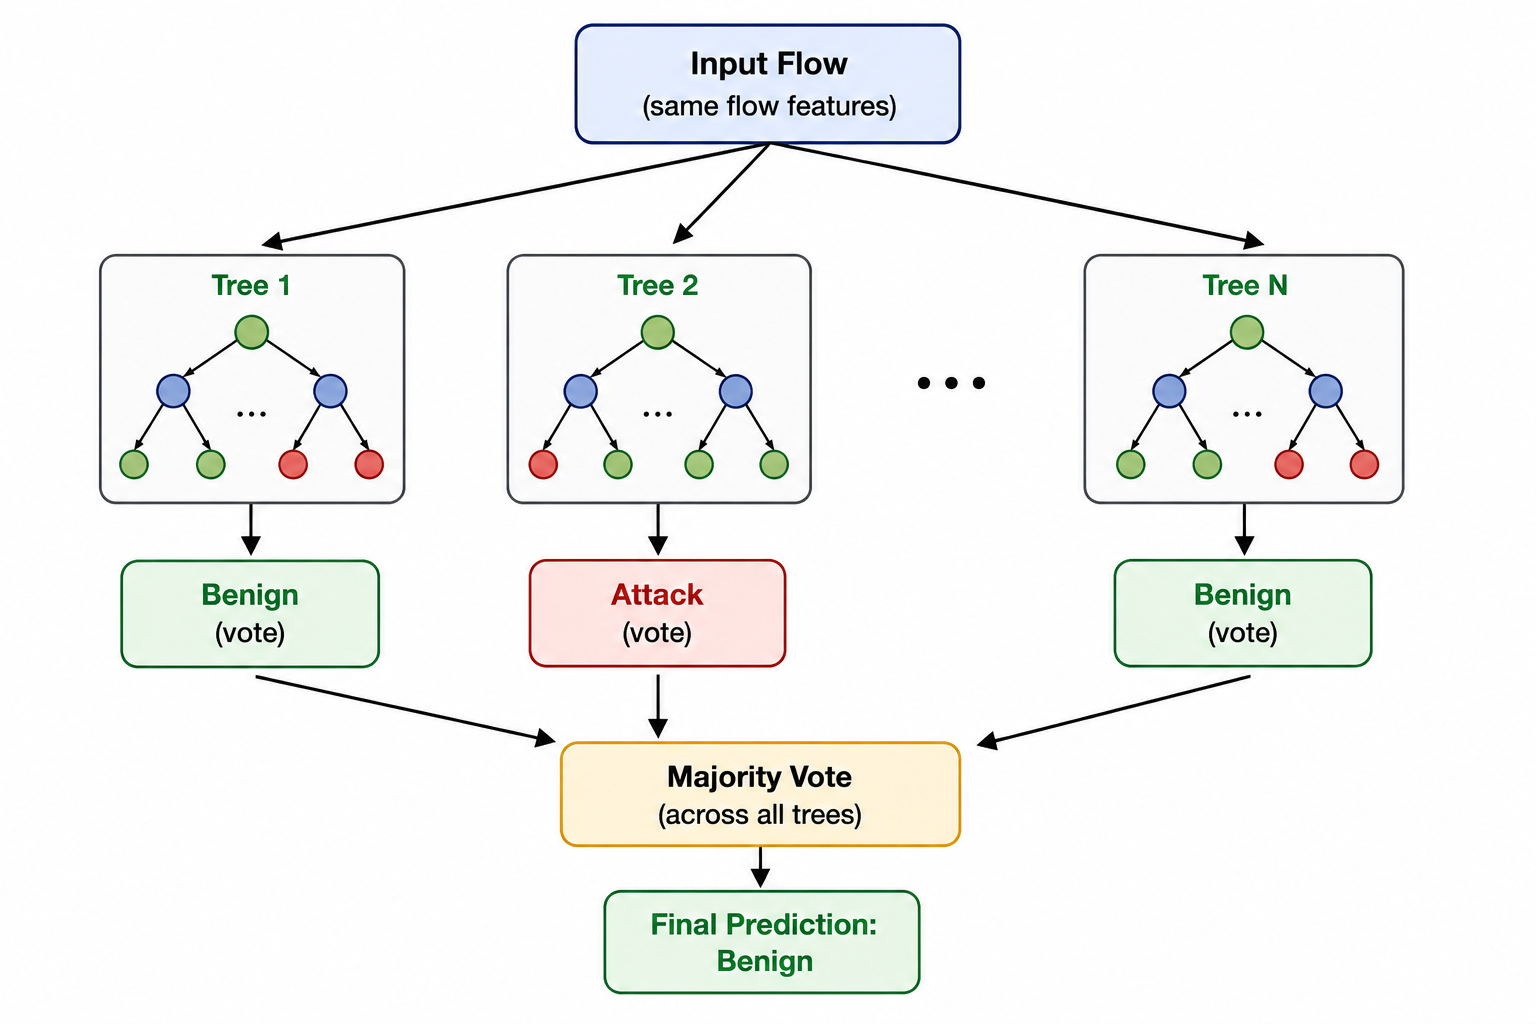
\includegraphics[width=0.8\textwidth]{figures/random_forest_voting.png}%
  }{%
    \fbox{\parbox{0.78\textwidth}{\centering\vspace{1.2cm}
    \texttt{[Figure: random\_forest\_voting.png, to be created]}\\[4pt]
    \small A simple original diagram: one input flow at the top, an arrow fanning
    out to several small decision-tree icons (Tree 1, Tree 2, ... Tree N), each
    producing its own Attack/Benign vote, all arrows converging into a single
    "Majority Vote" box at the bottom producing the final label. Draw in draw.io,
    PowerPoint, or a tikzpicture.
    \vspace{1.2cm}}}%
  }
  \caption{How a Random Forest reaches a decision \cite{breiman2001random}.}
  \label{fig:random_forest}
\end{figure}
 
Randomness is what matters, by making the trees less correlated with each other, we ensure that the error of any particular tree has a tendency to be offset by the errors of the others, which is more helpful for the result as compared to those errors accumulating over the ensemble of trees, ultimately yielding a classifier that performs at about the same speed and is as interpretable as a single decision tree while having the advantages of both increased robustness and accuracy. Besides this, Random Forest is capable of producing feature importance scores that rank features by how they contribute to the overall accuracy of the classifier which is useful for identifying drivers for detections, something that will be addressed again in Section~\ref{sec:xai}. Therefore, Random Forest will be our base classifier, although not as advanced as other techniques, it represents a sound choice due to the good trade off it presents in terms of complexity, speed and interpretability. The choice also sits on familiar ground: the decision trees a forest is built from were found by Alloghani et al. \cite{alloghani2020systematic} to be among the most implemented and discussed supervised learners in the applied literature.

\subsection{A brief word on other classical methods}
 
There are two other algorithms that appear frequently enough in the IDS literature that are worth mentioning very briefly. The Support Vector Machine \cite{cortes1995svm}, which was pioneered by Cortes and Vapnik, maps the input data into a higher-dimensional space and finds the smoothest possible separating plane which divides the two class labels with the largest possible margin. The k-Nearest Neighbour \cite{cover1967knn}, which is among the oldest rules for classification, works by going over all of the training examples already seen and determining the label of the ones that most closely resemble the new input data. Although both techniques are of interest, neither is a key component in this work, so they aren't addressed in any detail in the remaining chapters.
 
% ────────────────────────────────────────────────────────────
\section{Neural Networks and Deep Learning}
\label{sec:deep_learning}

“Deep” just means deep in a literally visual sense of stacking dozens or more levels of simple compute on top of one another, where each layer process input from the previous layer just a little and after passing through many such layers the data eventually is being described in a format where making the final choice is easy.   LeCun, Bengio, and Hinton, in a summary designed for a broad scientific audience, summarized it quite aptly: for supervised deep learning of the typical kind, a device is fed many instances with an associated label, outputs a value corresponding to each possible classification label, and fine-tunes its parameters every time the score does not correspond to the label \cite{lecun2015deep}. For a general neural network for classification, this applies to nearly everything in terms of image or network flow classification.
 
\subsection{Why neural networks took over}
 
The simple answer: scale. Machine learning approaches that are good with structured, already organized data the tabular structure of the CICFlowMeter output, for example are more straightforward: models like Random Forest can learn relationships that the provided table implicitly describes. Neural nets, on the other hand, are much more at home dealing with something more closely resembling raw input: you can feed a net raw pixels from an image or a stream of values, and it can learn the relevant characteristics on its own. 

LeCun, Bengio, and Hinton refer to it this way: rather than designing a feature extractor using domain knowledge to identify what information to extract for an input (for example, a dog image is useful if you look for ear shapes and dog nose), representation learning can find the right representation for an input automatically \cite{lecun2015deep}. 

When there was enough data, enough compute power and enough interest in training networks this way, it was the power of these nets to find their own relevant features that enabled rapid advances in areas like image recognition, after a 2012 paper radically reduced the error rate of a popular image benchmark \cite{krizhevsky2012imagenet}. We’ve since been trying to apply those same advances to network data.
 
\subsection{Convolutional networks}
 
CNN (Convolutional Neural Network): is a type of neural network, not scanning every individual input value separately, but scanning for small patterns locally in the input. In a word from O'Shea and Nash's tutorial, the same little filter is moved all the way over the input. So as soon as that local pattern appears on the image anywhere the same filter recognizes it. The network doesn't have to relearn that same pattern independently in every different location, and this is where much of the CNN’s effectiveness in image-based tasks comes from \cite{oshea2015cnn}” Although this structure is motivated by images, it maps perfectly to network data, where a pattern would appear as a short burst of unusual packet flow.

\subsection{Sequence aware networks}
 
Network traffic is not simply a bunch of unrelated flow requests-the order that flows happen often is meaningful. A “slow” port scan doesn’t result in any single flow request of significant size; it only looks out of the ordinary when you analyze a series of such flows over time. Sequence modeling architectures, most importantly LSTMs (Long Short-Term Memory), do carry information between steps. 

As proposed in 1997 by Hochreiter and Schmidhuber \cite{hochreiter1997lstm}, the architecture helps deal with the tendency of many-steps-ago information to vanish before affecting a future step’s decision by using its “gates” mechanism that allow useful information to be maintained. 

An architecture like the CNN presented here is not able to retain memory this way; however, you should know this architecture as it has been used in some systems such as the ones in Chapter~\ref{chap:ids}.

\subsection{The trade-off neural networks bring}
 
However, none of this is without cost. Neural networks tend to require significantly more training data to get anywhere close to top performance, also tend to take significantly longer to train and, most importantly for the purpose of this project, tend to be much harder to interpret. A Random Forest might be able to provide you with a sense for why the decisions were made, whereas the inner workings of a neural network is (out of the box) a mystery. Table~\ref{tab:classical_vs_deep} summarizes this compromise more quantitatively.
 
\begin{table}[H]
  \centering
  \caption{Classical machine learning vs.\ deep learning}
  \label{tab:classical_vs_deep}
  \renewcommand{\arraystretch}{1.4}
  \begin{tabularx}{\textwidth}{lXX}
    \toprule
    \textbf{Factor} & \textbf{Classical ML (e.g.\ Random Forest)} & \textbf{Deep
      learning (e.g.\ CNN, LSTM)} \\
    \midrule
    Data to be trained & Performs best on medium sized labeled data sets &
      Usually requires a significantly bigger data set to be effective \\
    Feature engineering & Needs features pre-computed (ex: using CICFlowMeter) & Can extract useful information from minimally processed data \\
    Training time & Fast minutes on a standard CPU & This typically takes several hours, although requires a GPU for training in a practical time frame. \\
    Interpretability & High decision paths, feature importance directly visible & Low by default: you have to add another Explainable Method (e.g. SHAP). \\
    Traditional IDS applications & Good as a strong baseline; works well for \\
    flow-level tabular features. & Better for sequential attacks / attacks over time \\
    \bottomrule
  \end{tabularx}
\end{table}
 
The training-data and training-time rows are what Ahmad et al. Noticed about the deep learning IDS work they reviewed-that deep models usually had GPU test beds, sizable data-sets, and comparable accuracy \cite{ahmad2021network}. The interpretability row is a key insight from Lundberg and Lee: the most accurate models on sizable data-sets often are precisely the models most difficult for a person to interpret \cite{lundberg2017shap}. No row is definitively "better"-they’re appropriate in different parts of the process and it’s the value of that trade-off which has given rise to explainability methods, introduced next.

\section{Making Model Decisions Understandable}
\label{sec:xai}
 
A system that achieves 99\% accuracy but provides no explanation for any of its classifications is of limited value to security professionals. If the system determines a connection is malicious, for instance, the analyst will require some understanding of why the connection was deemed malicious before acting on it, whether that’s by blocking a particular IP, escalating an incident to the next level, or dismissing the alert as a false positive. The exact same dilemma is articulated in the context of intrusion detection systems (IDS) in the 2025 systematic literature review on XAI adoption in IDS by Mohale and Obagbuwa, who point out that many of today’s most accurate IDS are black boxes, obscuring the reasons behind alerted events and hampering analyst trust in these systems \cite{mohale2025xaiids}. This practical impediment is precisely what lies behind XAI, and is highly pertinent to the objectives of this research of developing an explainability layer within the detection workflow.
 
\subsection{The problem in plain terms}
 
Lundberg and Lee pose the problem most directly: The top accuracy on large, modern
datasets usually come from models that people are the least capable of interpreting, which generates a tension between model performance and human interpretability \cite{lundberg2017shap}. You wouldn’t get from hundreds of trees in a Random Forest, or millions of internal parameters in a neural network, a one-sentence answer explaining any single prediction. You have to apply something else on top, after the fact.
 
\subsection{SHAP values}

The method the project employs is called SHAP (SHapley Additive exPlanations). This concept is adapted from a far older game-theory method that helps you to divide the credit among individuals who worked to achieve some collective result. SHAP implements this for the features of a model and, for any given prediction, computes the extent to which each input feature has shifted the result towards the output "attack" class (and away from "benign"), summing exactly to the final prediction \cite{lundberg2017shap}.

This translates, in a practical sense, to this system not simply reporting an alert: if the detection system alerts that a flow is malicious, then in addition to the classification, it will explain precisely why: the flow was flagged because the number of SYN packets was far higher than normal and the connection was far shorter than normal, for example. This ability to decompose why an alert has occurred is how one can transition a black box to a set of decisions a security analyst can meaningfully make and that is the main contribution here.
% ────────────────────────────────────────────────────────────
\section{Summary}
 
Replacing hard coded detection rules with data derived patterns comes in the form of machine learning where a particular flavour will depend on whether you can provide examples with expected outputs (supervised learning) or you cannot (unsupervised learning). There’s quite more to building a functional model than just training it. You will need to collect data, turn it into meaningful features, partition the data for testing, and finally assess the models with metrics that actually have a real bearing on the problem, which in this case means high recall and precision (not accuracy).

My default model, given its speed, familiarity, and truly decent performance (even without tuning) is an ensemble of decision trees, aka a Random Forest. I would like to explore a few Deep Learning solutions, a Convolutional Neural Network (CNN), and a “time aware” one, called Long Short-Term Memory (LSTM), which will most likely require a higher volume of training data but has also proven capabilities for this problem. SHAP value can bring back interpretability lost in those deeper models.
Based on that foundations I will explore the different machine learning approaches to network intrusion detection, focusing on what works and what doesn’t and where is there space to improvement that my projects hopes to address.
